\chapter{实验结果}\label{sec:experiment}

\section{短视频应用系统}
本系统选用 Spring Framework、Spring MVC 以及 MyBatis 框架实现。最终系统功能为用户注册、登录、发布视频、观看视频、视频点赞、关注用户、发表评论。

\subsection{用户登录、注册}
如图 \ref{fig:LoginRegister} 所示,本系统的登录与注册页面较为相似,用户在登录页面输入用户名密码后即可登录,且登录信息自动保存五天,五天内可不登录使用。登录成功后页面会自动跳转到应用首页。注册页面用户需输入系统内唯一的用户名和一个强密码,注册成功后会跳转到个人信息完善界面。

\begin{figure}[!ht]
\centering
\subfloat[登录页面]{
	\centering
	
\includegraphics[width=0.2\textwidth]{weapp1}}\quad\quad
\subfloat[注册页面]{
	\centering
	
\includegraphics[width=0.2\textwidth]{weapp2}}
\caption{应用登录与注册页面}
\label{fig:LoginRegister}
\end{figure}


\subsection{发布、观看视频}

如图 \ref{fig:index} 所示,用户在登录后即可在首页点击视频以进入视频详情页观看视频。用户可以在首页通过底部的功能栏快速执行搜索、发布视频、查看关注视频以及查看个人信息等功能。用户在首页也可以点击视频作者的头像进入作者个人信息页。


\begin{figure}[!ht]
\centering
\subfloat[首页]{
	\centering
	
\includegraphics[width=0.2\textwidth]{weapp4}}\quad\quad
\subfloat[视频详情页]{
	\centering
	
\includegraphics[width=0.2\textwidth]{weapp5}}\quad\quad
\subfloat[视频发布页]{
	\centering
	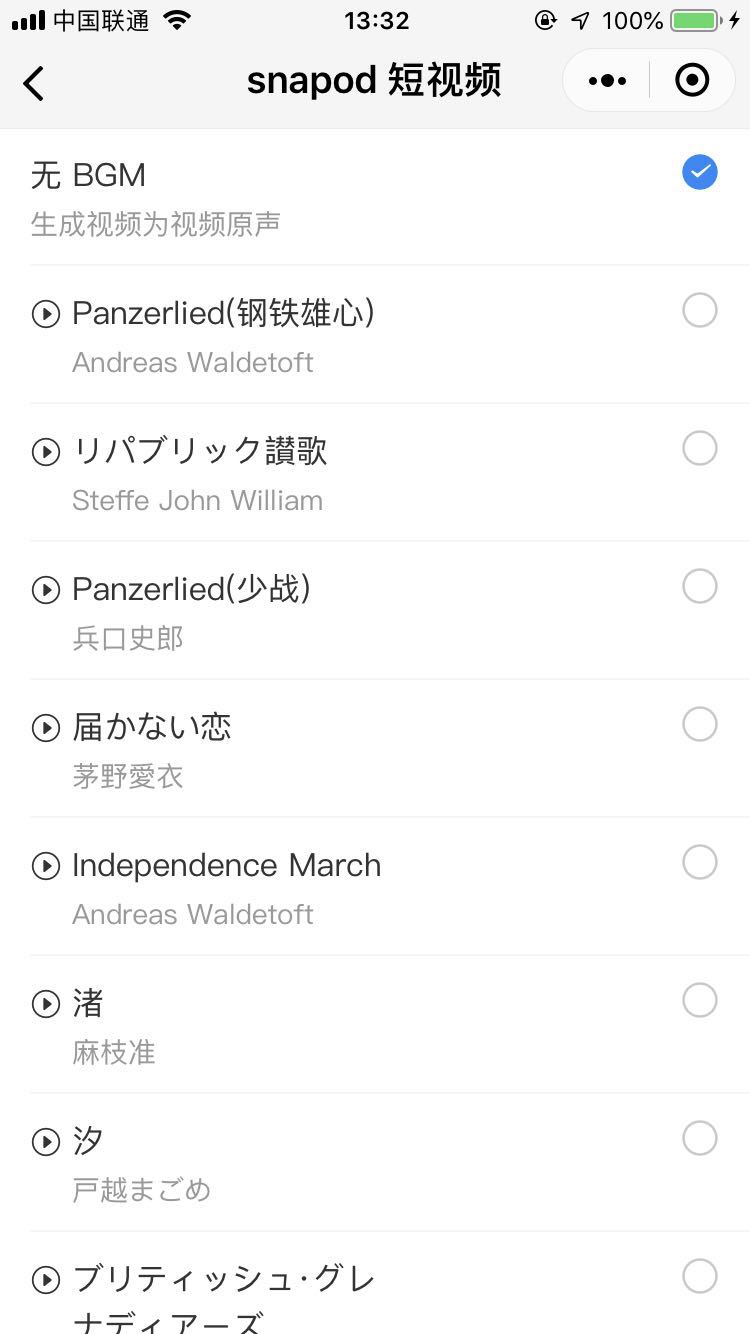
\includegraphics[width=0.2\textwidth]{weapp3}}
\caption{应用首页、视频详情页以及视频发布页}
\label{fig:index}
\end{figure}

用户在视频详情页可以观看视频,并对视频作出操作如快速进入视频发布页、快速进入搜索页面、进入视频作者个人信息界面、视频点赞、评论、转发、回到首页进入自己个人信息页面等操作。

用户可以选择使用相机拍摄视频或从相册中选择视频,用户选择完视频后进入视频发布页。用户在视频发布页可以选择视频背景音乐和视频描述信息。用户选择发布后,视频会被上传到服务端进行处理,处理完毕后即可在线观看。

\subsection{视频点赞、关注用户与发表评论}

用户可以对一个视频进行点赞以及关注某一个用户。如图 \ref{fig:LikeWatch} 所示,用户在点赞某视频后可以在自己的个人页面中的收藏夹找到。用户在关注某个用户后可以在自己个人页面的关注栏中找到关注用户发布的所有视频。

\begin{figure}[!ht]
\centering
\subfloat[用户关注栏]{
	\centering
	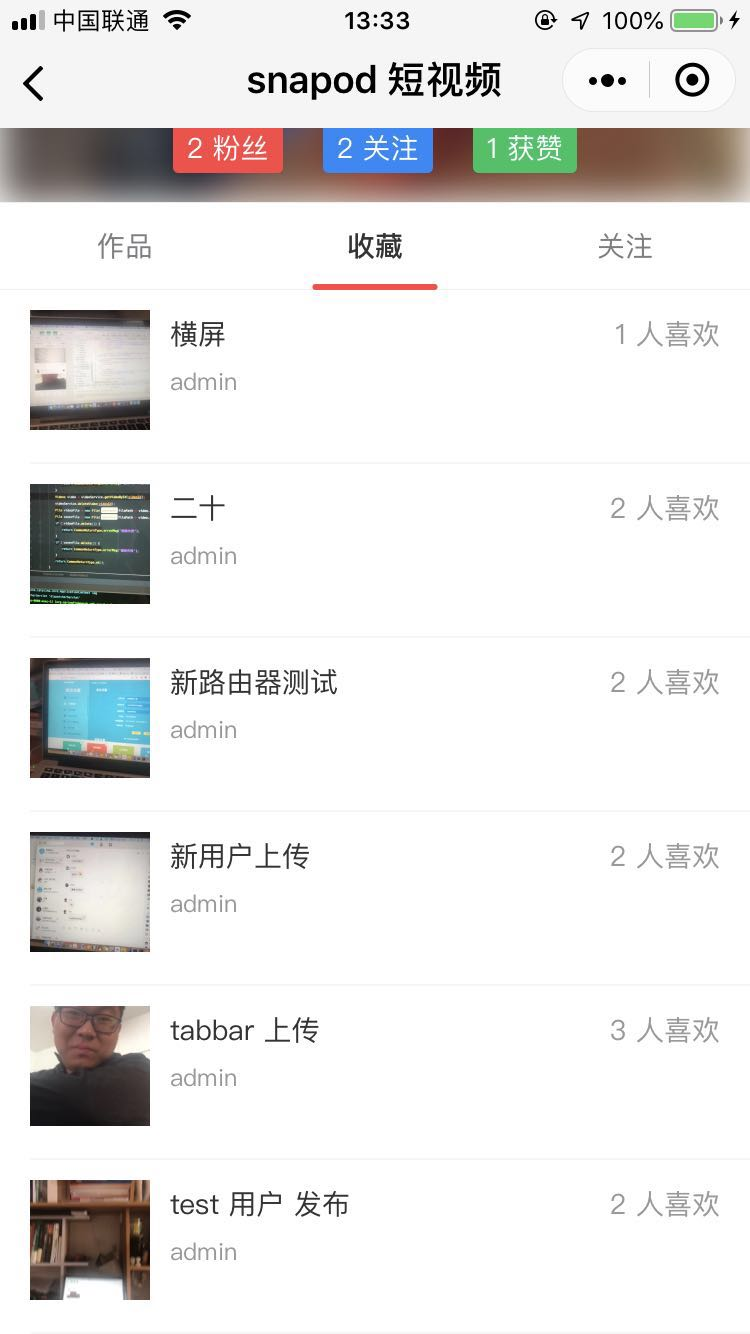
\includegraphics[width=0.2\textwidth]{weapp6}}\quad
\subfloat[用户收藏栏]{
	\centering
	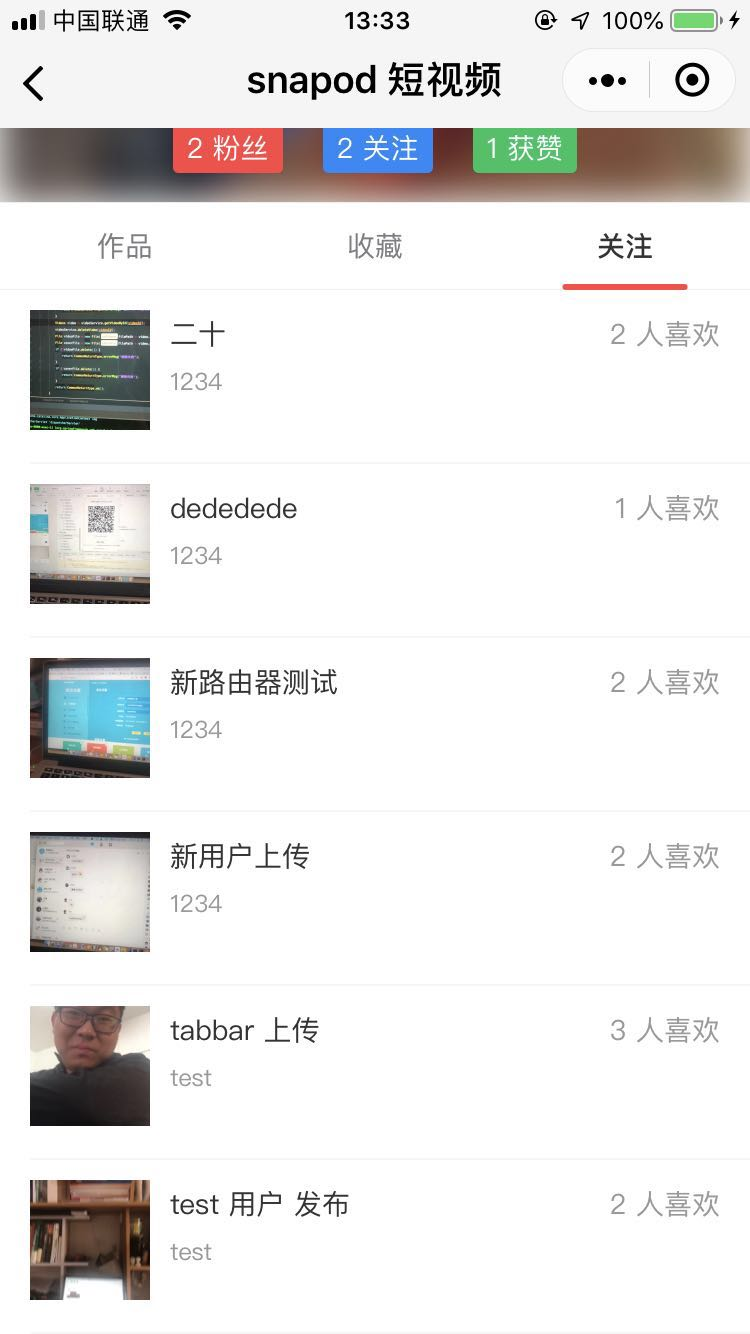
\includegraphics[width=0.2\textwidth]{weapp7}}\quad
\subfloat[视频评论]{
	\centering
	
\includegraphics[width=0.2\textwidth]{weapp8}}
\caption{视频收藏、用户关注与视频评论}
\label{fig:LikeWatch}
\end{figure}

用户在视频详情页中点击评论按钮即可弹出视频的评论信息。如图 \ref{fig:LikeWatch} 所示,视频评论信息包含了对于该视频的所有的评论,用户可以发布视频的评论也可以对某一个评论进行回复。

%\subsection{发表评论}
%
%用户在视频详情页中点击评论按钮即可弹出视频的评论信息。如图 \ref{fig:comments} 所示,视频评论信息包含了对于该视频的所有的评论,用户可以发布视频的评论也可以对某一个评论进行回复。
%
%\begin{figure}[!ht]
%    \centering
%    
\includegraphics[width=0.5\textwidth]{weapp8}
%    \caption{视频评论信息}
%    \label{fig:comments}
%\end{figure}



\section{SQL 优化结果}
SQL 优化包括参数优化和具体查询优化两部分。

\subsection{参数优化}
参数优化主要是根据基准测试对数据库做出的全局优化如调整缓存、日志输出等设置。参数优化的效果主要是通过数据库系统的基准测试体现的,这里使用 sysbench\cite{sysbench2019} 提供的在线事务 (OLTP) 测试功能来模拟一个在线电商服务的数据库读取情况进行数据库系统的基准测试。数据库系统基准测试主要测试标准有数据库每秒钟处理事务数 (tps),数据库系统每秒钟处理查询数 (qps) 以及数据库查询延迟。

基准测试采用在线事务读写测试,采用 32 个线程并发读写,测试数据库包含 10 张数据表,每个数据表包含 300000 条数据,基准测试时间为 1800 秒。进行数据库参数优化之前,基准测试结果为读取数据库 4401670 次,平均写入数据库 1257610 次,每秒处理事务数为 174.63,平均每秒处理查询数为 3492.62,平均查询延迟为 511.33 毫秒。由于服务器性能以及没有优化的原因,测试结果表现较差。每秒处理事务数、每秒处理查询数以及延迟时间变化情况如图 \ref{fig:bench_result} 所示。

\begin{figure}[!ht]
	\centering
	\subfloat[TPS]{
	 \centering
	 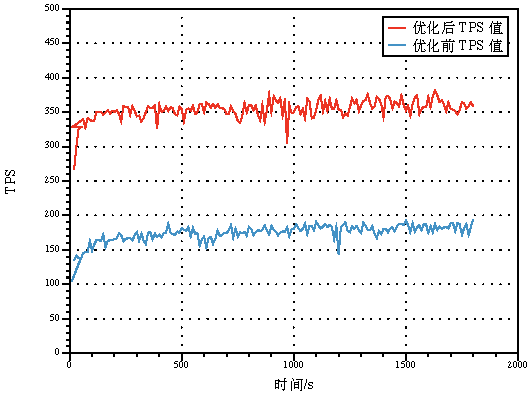
\includegraphics[scale=0.8]{tps_compare.pdf}}\quad
 \subfloat[QPS]{
	 \centering
	 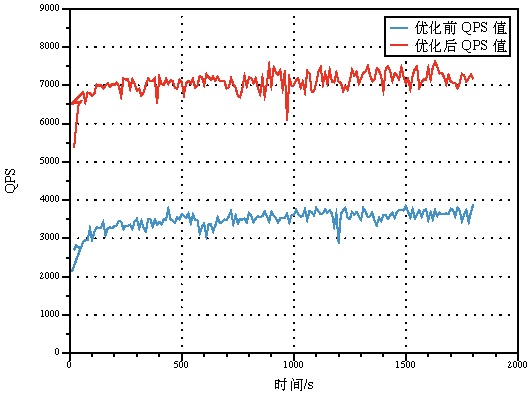
\includegraphics[scale=0.8]{qps_compare.pdf}}\quad
 \subfloat[延迟时间]{
	 \centering
	 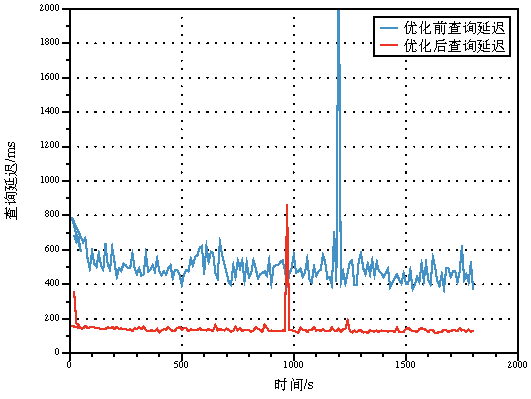
\includegraphics[scale=0.8]{lat_compare.pdf}}
	\caption{优化前后数据库基准测试结果}
	\label{fig:bench_result}
 \end{figure}

对基准测试结果以及进行基准测试时数据库系统对资源的占用情况进行分析,数据库在进行大量数据并发读写时对磁盘利用率过高。这可能由于more的 innodb 储存引擎缓冲过小,频繁触发 innodb 最大脏页的限制,导致磁盘占用过高,优化可以从调整缓存大小以及优化日志文件等方面进行。由于本系统并不涉及很高的安全性同时每次事务提交都比较小,所以可以将 innodb\_flush\_log\_at\_trx\_commit\cite{姜承尧2011mysql} 属性设置为 0 或 2,来降低磁盘读写。最后通过改变存储引擎双写入缓冲设置来避免双写入缓冲。优化后,基准测试结果岁时间变化图如图  所示。经过优化后,数据库平均每秒处理事务数为 353.92,平均每秒处理查询数为 7078.34,平均查询延迟时间为 139.85毫秒。可见,优化后各项数据均有比较明显的提升,优化操作对数据库行呢个提升有非常大的帮助。

\subsection{查询优化}

进行查询优化前的元查询为通过嵌套查询与自然连接的方式实现。通过数据库 explain\cite{mysql2019} 命令分析得出的查询执行计划如表 \ref{tab:pre_explain} 所示,数据库在执行该查询时创建了一个临时表,同时由于查询属性上没有设置索引,数据库对用户与用户视频关系进行了全表扫描,效率较低,查询速度很慢。
\begin{table}[!ht]
    \centering
    \caption{优化前查询语句查询方案分析表}
	\label{tab:pre_explain}
	\footnotesize
	\begin{tabularx}{\textwidth}{cccccccc}
    \toprule
    编号 & 查询类型 & 查询表 & 执行类型 & 可能使用索引 & 实际使用索引 & 估计查找行数 & 备注  \\ \midrule
    1 & SIMPLE & <subquery3> & ALL & NULL & NULL & NULL & NULL \\
    1 & SIMPLE & videos & eq\_ref & PRIMARY & PRIMARY & 1 & NULL \\
    1 & SIMPLE & u & ALL & NULL & NULL & 99803 & Using where; \\ 
    3 & MATERIALIZED & user\_like\_videos & ALL & NULL & NULL & 223167 & Using where; \\ \bottomrule
    \end{tabularx}
\end{table}

对于查询创建临时表以及查询属性没有索引的问题可以使用数据库的内连接操作代替嵌套查询以及在相应属性列上建立索引来解决。使用数据库的内连接操作将原先的嵌套查询语句进行重构,并在所有的查询属性上建立 B-Tree 索引来加速查找。修改过后该插叙语句的执行计划如表 \ref{tab:af_explain} 所示,优化过后查询没有产生临时表,且所有的表在查找时都用到了索引,查询次数大大减小,效率也提高了。

\begin{table}[!ht]
    \centering
    \caption{优化后查询语句查询方案分析表}
	\label{tab:af_explain}
	\small
    \begin{tabularx}{\textwidth}{cccccccc}
    \toprule
    编号 & 查询类型 & 查询表 & 执行类型 & 可能使用索引 & 实际使用索引 & 估计查找行数 & 备注  \\ \midrule
    1 & SIMPLE & u & const & PRIMARY, unique\_id & PRIMARY & 1 & NULL \\
    1 & SIMPLE & ulv & ref & user & user & 29870 & NULL; \\ 
    1 & SIMPLE & v & eq\_ref & PRIMARY & PRIMARY & 1 & Using where; \\ \bottomrule
    \end{tabularx}
\end{table}


在包含十万个测试用户、一百万个测试视频以及三十万个测试用户视频关系的数据库中进行测试,优化前语句执行速度为 277.64 秒,这样的速度显然是不能接受的,优化后查询执行速度达到了 1.75 秒,可见优化对于查询语句执行速度提升的效果非常明显。


\section{视频编码优化结果}
优化前采用 x264 作为视频编码器,参数设置为视频分辨率为 $1920\times1080$、视频帧率为 29.97 帧以及视频码率设置为 4Mbps。测试视频为 $1920\times1080$ 分辨率、60 帧、时长 10秒的手机拍摄视频。优化前压制时间为 26.3 秒,压制后视频平均相对原视频失真即 平均PSNR 为 39.96。优化后,视频编码器采用支持硬件加速的 h264\_videotoolbox 编码器、使用 CPU 核心显卡进行硬件加速。视频压制参数设置为 视频分辨率为 $1920\times1080$、视频帧率为 29.97 帧、视频码率设置为 4Mbps、视频 prifile 设置为 High 、压制时采用 h264 编码的 medium 预设以及由于短视频长度较短,用户不太可能拉动视频进度条,所以增大默认的关键帧间隔,测试视频不变。优化后,压制视频所需时间为 4.34 秒、平均 PSNR 为 39.28。可见优化在视频失真度基本不变时,大大降低了压制视频所需时间。

\section{本章小结}
本章叙述了系统开发结果与数据库和视频压制优化的具体作用。由最终结果可知本系统开发过程中各种优化措施均起到了一定的作用。
